%%%% Dokumentklassen %%%%

\documentclass[a4paper,11pt,fleqn,dvipsnames,twoside,openright]{memoir} 	% Openright åbner kapitler på højresider (openany begge)


%%%% PACKAGES %%%%

%% Oversættelse og tegnsætning %%
\usepackage[utf8]{inputenc}					% Input-indkodning af tegnsæt (UTF8)
\usepackage[danish]{babel}					% Dokumentets sprog
\usepackage[T1]{fontenc}					    % Output-indkodning af tegnsæt (T1)
\usepackage{ragged2e,anyfontsize}			% Justering af elementer
\usepackage{fixltx2e}						% Retter forskellige fejl i LaTeX-kernen
																			
%% Figurer og tabeller (floats) %%
\usepackage{graphicx} 						% Håndtering af eksterne billeder (JPG, PNG, EPS, PDF)
\usepackage{multicol}         	            	% Muliggør output i spalter
\usepackage{rotating}						% Rotation af tekst med \begin{sideways}...\end{sideways}
\usepackage{xcolor}							% Definer farver med \definecolor. Se mere: http://en.wikibooks.org/wiki/LaTeX/Colors
\usepackage{flafter}						% Sørger for at floats ikke optræder i teksten før deres reference
\let\newfloat\relax 						% Justering mellem float-pakken og memoir
\usepackage{float}							% Muliggør eksakt placering af floats, f.eks. \begin{figure}[H]

%% Matematik mm. %%
\usepackage{amsmath,amssymb,stmaryrd} 		% Avancerede matematik-udvidelser
\usepackage{mathtools}						% Andre matematik- og tegnudvidelser
\usepackage{textcomp}                 		% Symbol-udvidelser (fx promille-tegn med \textperthousand)
\usepackage{rsphrase}						% Kemi-pakke til RS-saetninger, fx \rsphrase{R1}
\usepackage[version=3]{mhchem} 				% Kemi-pakke til flot og let notation af formler, f.eks. \ce{Fe2O3}
\usepackage{siunitx}						% Flot og konsistent præsentation af tal og enheder med \si{enhed} og \SI{tal}{enhed}
\sisetup{output-decimal-marker = {,}}		% Opsætning af \SI (DE for komma som decimalseparator) 

%% Referencer og kilder %%
\usepackage[danish]{varioref}				% Muliggør bl.a. krydshenvisninger med sidetal (\vref)
\usepackage{natbib}							% Udvidelse med naturvidenskabelige citationsmodeller
\usepackage{xr}							    % Referencer til eksternt dokument med \externaldocument{<NAVN>}

%% Misc. %%
\usepackage{listings}						% Placer kildekode i dokumentet med \begin{lstlisting}...\end{lstlisting}
\usepackage{lipsum}							% Dummy text \lipsum[..]
\usepackage[shortlabels]{enumitem}			% Muliggør enkelt konfiguration af lister
\usepackage{pdfpages}						% Gør det muligt at inkludere pdf-dokumenter med kommandoen \includepdf[pages={x-y}]{fil.pdf}	
\pdfoptionpdfminorversion=6					% Muliggør inkludering af pdf-dokumenter, af version 1.6 og højere
\pretolerance=2500 							% Justering af afstand mellem ord (højt tal, mindre orddeling og mere luft mellem ord)	


%%%% CUSTOM SETTINGS %%%%

%% Marginer %%
\setlrmarginsandblock{3.5cm}{2.5cm}{*}		% \setlrmarginsandblock{Indbinding}{Kant}{Ratio}
\setulmarginsandblock{2.5cm}{3.0cm}{*}		% \setulmarginsandblock{Top}{Bund}{Ratio}
\checkandfixthelayout 						% Oversætter værdier til brug for andre pakker

%% Afsnitsformatering %%
\setlength{\parindent}{0mm}           		% Størrelse af indryk
\setlength{\parskip}{3mm}          			% Afstand mellem afsnit ved brug af double Enter
\linespread{1,1}							% Linjeafstand

%% Indholdsfortegnelse %%
\setsecnumdepth{subsection}		 			% Dybden af nummererede overskrifter (part/chapter/section/subsection)
\maxsecnumdepth{subsection}					% Dokumentklassens grænse for nummereringsdybde
\settocdepth{subsection} 					% Dybden af indholdsfortegnelsen
		
%% Opsætning af listings %%
\definecolor{commentGreen}{RGB}{34,139,24}
\definecolor{stringPurple}{RGB}{208,76,239}

\lstset{language=Matlab,					    % Sprog
	basicstyle=\ttfamily\scriptsize,		    % Opsætning af teksten
	keywords={for,if,while,else,elseif,		% Nøgleord at fremhæve
			  end,break,return,case,
			  switch,function},
	keywordstyle=\color{blue},				% Opsætning af nøgleord
	commentstyle=\color{commentGreen},		% Opsætning af kommentarer
	stringstyle=\color{stringPurple},		% Opsætning af strenge
	showstringspaces=false,					% Mellemrum i strenge enten vist eller blanke
	numbers=left, numberstyle=\tiny,		    % Linjenumre
	extendedchars=true, 					    % Tillader specielle karakterer
	columns=flexible,						% Kolonnejustering
	breaklines, breakatwhitespace=true,		% Bryd lange linjer
}

%% Navngivning %%
\addto\captionsdanish{
	\renewcommand\appendixname{Appendiks}
	\renewcommand\contentsname{Indholdsfortegnelse}	
	\renewcommand\appendixpagename{Appendiks}
	\renewcommand\appendixtocname{Appendiks}
	\renewcommand\cftchaptername{\chaptername~}		% Skriver "Kapitel" foran kapitlerne i indholdsfortegnelsen
	\renewcommand\cftappendixname{\appendixname~}	% Skriver "Appendiks" foran appendiks i indholdsfortegnelsen
}

%% Kapiteludssende %%
\definecolor{numbercolor}{gray}{0.7}		            % Definerer en farve til brug til kapiteludseende
\newif\ifchapternonum

\makechapterstyle{jenor}{					        % Definerer kapiteludseende frem til ...
  \renewcommand\beforechapskip{0pt}
  \renewcommand\printchaptername{}
  \renewcommand\printchapternum{}
  \renewcommand\printchapternonum{\chapternonumtrue}
  \renewcommand\chaptitlefont{\fontfamily{pbk}\fontseries{db}\fontshape{n}\fontsize{25}{35}\selectfont\raggedleft}
  \renewcommand\chapnumfont{\fontfamily{pbk}\fontseries{m}\fontshape{n}\fontsize{1in}{0in}\selectfont\color{numbercolor}}
  \renewcommand\printchaptertitle[1]{%
    \noindent
    \ifchapternonum
    \begin{tabularx}{\textwidth}{X}
    {\let\\\newline\chaptitlefont ##1\par} 
    \end{tabularx}
    \par\vskip-2.5mm\hrule
    \else
    \begin{tabularx}{\textwidth}{Xl}
    {\parbox[b]{\linewidth}{\chaptitlefont ##1}} & \raisebox{-15pt}{\chapnumfont \thechapter}
    \end{tabularx}
    \par\vskip2mm\hrule
    \fi
  }
}											        % ... her

\chapterstyle{jenor}						        % Valg af kapiteludseende - Google 'memoir chapter styles' for alternativer

%% Sidehoved %%

\makepagestyle{AAU}							        % Definerer sidehoved og sidefod udseende frem til ...
\makepsmarks{AAU}{%
	\createmark{chapter}{left}{shownumber}{}{. \ }
	\createmark{section}{right}{shownumber}{}{. \ }
	\createplainmark{toc}{both}{\contentsname}
	\createplainmark{lof}{both}{\listfigurename}
	\createplainmark{lot}{both}{\listtablename}
	\createplainmark{bib}{both}{\bibname}
	\createplainmark{index}{both}{\indexname}
	\createplainmark{glossary}{both}{\glossaryname}
}
\nouppercaseheads									% Ingen Caps ønskes

\makeevenhead{AAU}{\small ST3PRJ3 Gruppe X}{}{\leftmark}	% Definerer lige siders sidehoved (\makeevenhead{Navn}{Venstre}{Center}{Hoejre})
\makeoddhead{AAU}{\rightmark}{}{\small ASE}		            % Definerer ulige siders sidehoved (\makeoddhead{Navn}{Venstre}{Center}{Højre})
\makeevenfoot{AAU}{\small \thepage}{}{}						% Definerer lige siders sidefod (\makeevenfoot{Navn}{Venstre}{Center}{Højre})
\makeoddfoot{AAU}{}{}{\small \thepage}						% Definerer ulige siders sidefod (\makeoddfoot{Navn}{Venstre}{Center}{Højre})

\copypagestyle{AAUchap}{AAU}							% Sidehoved for kapitelsider defineres som standardsider, men med blank sidehoved
\makeoddhead{AAUchap}{}{}{}
\makeevenhead{AAUchap}{}{}{}
\makeheadrule{AAUchap}{\textwidth}{0pt}
\aliaspagestyle{chapter}{AAUchap}					% Den ny style vælges til at gælde for chapters
													% ... her
															
\pagestyle{AAU}										% Valg af sidehoved og sidefod


%%%% CUSTOM COMMANDS %%%%

%% Billede hack %%
\newcommand{\figur}[4]{
		\begin{figure}[H] \centering
			\includegraphics[width=#1\textwidth]{billeder/#2}
			\caption{#3}\label{#4}
		\end{figure} 
}

%% Specielle tegn %%
\newcommand{\decC}{^{\circ}\text{C}}
\newcommand{\dec}{^{\circ}}
\newcommand{\m}{\cdot}


%%%% ORDDELING %%%%

\hyphenation{}


%%%% Tilføjelser af min preample %%%%

% Booktabs:
% The booktabs package is needed for better looking tables. 
\usepackage{booktabs}

% Caption:
% For better looking captions. See caption documentation on how to change the format of the captions.
\usepackage[hang, font={small, it}]{caption}

% Hyperref:
% This package makes all references within your document clickable. By default, these references will become boxed and colored. This is turned back to normal with the \hypersetup command below.
\usepackage{hyperref}
	\hypersetup{colorlinks=false,pdfborder=0 0 0}

% Cleveref:
% This package automatically detects the type of reference (equation, table, etc.) when the \cref{} command is used. It then adds a word in front of the reference, i.e. Fig. in front of a reference to a figure. With the \crefname{}{}{} command, these words may be changed.
\usepackage{cleveref}
	\crefname{equation}{formel}{formler}
	\crefname{figure}{figur}{figurer}	
	\crefname{table}{tabel}{tabeller}

% Mine tilføjelser:
\usepackage{units}                        %% Bruges til at gøre fx 1/2 samlet med: \nicefrac{1}{2}.
\usepackage{tabu, longtable}              %% Bruges til tabeller.
\setlength{\tabulinesep}{1.5ex}           %% Definerer linjeafstand i tabeller.
\usepackage{enumerate}                    %% Bruges til lister.
\usepackage{tabto}                        %% Giver mulighed for TAB med fx \tabto{3em}.
\usepackage[hyphenbreaks]{breakurl}       %% Bruges til websiders url'er.
\renewcommand{\UrlFont}{                  %% Definerer url-font.
\small\ttfamily}                          %
\bibliographystyle{plain}                 %% Definere bibliografien. Ses til sidst i dokumentet i kapitlet Litteratur.
\raggedbottom

\externaldocument[D-]{Dokumentation}

\begin{document}
	
\frontmatter						% Nummereres med romerske tal.
\begin{titlingpage}
\begin{center}

~ \\[3cm]


\includegraphics[width=0.6\textwidth]{figurer/ASE}~\\[1cm]

\textsc{\LARGE Aarhus School of Engineering}\\[1.5cm]

\textsc{\Large Sundhedsteknologi}\\
\textsc{\Large 3. semesterprojekt}\\[0.5cm]

\noindent\makebox[\linewidth]{\rule{\textwidth}{0.4pt}}\\
[0.5cm]{\Huge Rapport}
\noindent\makebox[\linewidth]{\rule{\textwidth}{0.4pt}}

\end{center}

\textit{Gruppe 3} \newline
Helle Randeris (201407703) \newline
Joakim Lindhardt (201404067) \newline
Lars Holst (201408737) \newline
Rune Rask (201271001) \newline		 
Finja Jette Ralfs (201303659) \newline
Signe S. Vaaben (201310503)  


\textit{Vejleder} \newline
Titel\\
Navn: Thomas Nielsen\\
Universitet: Ingeniørhøjskolen Aarhus Universitet


\vfill

\begin{center}
{\large \today}
\end{center}


\end{titlingpage}
\begin{vplace}[0.6]
{\large \textit{Gruppemedlemmer}}
\\
\\

\noindent \begin{tabular}{ll}
	\makebox[3.0in]{\hrulefill} & \makebox[1.5in]{\hrulefill}\\
	Helle Randeris (201407703) & 16/12-15\\[8ex]% adds space between the two sets of signatures
	\makebox[3in]{\hrulefill} & \makebox[1.5in]{\hrulefill}\\
	Joakim Lindhardt (201404067) & 16/12-15\\[8ex]
	\makebox[3in]{\hrulefill} & \makebox[1.5in]{\hrulefill}\\
	Lars Holst (201408737) & 16/12-15\\[8ex]
	\makebox[3in]{\hrulefill} & \makebox[1.5in]{\hrulefill}\\
	Rune Rask (201271001) & 16/12-15\\[8ex]
	\makebox[3in]{\hrulefill} & \makebox[1.5in]{\hrulefill}\\
	Finja Jette Ralfs (201303659) & 16/12-15\\[8ex]
	\makebox[3in]{\hrulefill} & \makebox[1.5in]{\hrulefill}\\
	Signe S. Vaaben (201310503) & 16/12-15\\[8ex]
\end{tabular}
\\
\\
\\
{\large \textit{Vejleder}}
\\
\\
  
\noindent \begin{tabular}{ll}
	\makebox[3.0in]{\hrulefill} & \makebox[1.5in]{\hrulefill}\\
	Thomas Nielsen & 16/12-15\\[8ex]
\end{tabular}
\end{vplace}


\chapter{Resumé}

Et resumé af rapporten.

\chapter{Forkortelser}

\begin{longtabu} to \linewidth{@{}l X[j]@{}}
    Forkortelse &    Forklaring\\
    \toprule
    BT &    blodtryk\\
\label{forkort}
\end{longtabu}
\cleardoublepage		

\tableofcontents*                   % Indsætter en indholdsfortegnelse før Indledning.

\mainmatter                         % Her findes de nummererede kapitler modsat \frontmatter og \backmatter. Nummereres med arabiske tal.
\chapter{Indledning}

Oprids af gruppens produkt og dets kunnen.
\chapter{Projektformulering}\label{kapitel_Projektformulering}

\section{Projektformulering}
I projektet vil der blive arbejdet med design og udvikling af et blodtryksmålesystem med henblik på måling af blodtryk. Dette skal måles invasivt, dvs. systemet skal kunne tilsluttes patientens arterier via et væskefyldt kateter.
Der arbejdes med problemstillingen set fra et sundhedsfagligt aspekt, da produktet tiltænkes i brug på en operationsstue, hvor der ofte er behov for kontinuert at monitorere patientens blodtryk. Blodtrykket er en vigtig parameter til monitorering af patientens helbredstilstand. Blodtryksmålesystemet ses derfor som et redskab for det sundhedsfaglige personale.
Visionen for projektet er at udvikle et system, der kan tilsluttes det væskefyldte kateter og vise en blodtrykskurve på en skærm. 



\section{Præcisering}


Projektet kommer til at indeholde to primære elementer. Et elektronisk kredsløb, som forstærker signalet fra transduceren og filtrerer det med et indbygget analogt filter. Projektet bygges op af et program, udviklet i C$\#$, til at vise blodtrykket som funktion af tiden. Programmet skal kunne kalibrere blodtrykssignalet og foretage en nulpunktsjustering. Blodtryksmålingen kan ikke startes før nulpunktsjusteringen er foretaget. Derudover skal programmet indeholde et digitalt filter, som kan filtrere blodtrykket - dette filter skal kunne slås til/fra. Programmet skal kunne gemme de målte data i en database.
Der stræbes efter at opbygge systemet efter 3-lagsmodellen med præsentationlag, logiklag og datalag.  


\section{Målgruppe}
Blodtryksmålersystemet er tænkt udviklet til en operationsstue. Der er udviklet én skærm, hvor der både skal indskrives data og målingen skal foretages. Det er derfor en rimelig bred målskare af sundhedsfagligt personale der skal kunne bruge skærmen.
\begin{itemize}
\item Anæstesisygeplejersker- og læger
\item Operationssygeplejersker- og læger
\end{itemize}

 

\chapter{Baggrund}\label{kapitel_Baggrund}
Udarbejdelsen af gruppens produkt har krævet indsamling og forståelse af en vis viden inden for blodtryk og blodtryksmåling.
Væsentlige dele af denne viden præsenteres her i et afsnit med sundhedsfaglig teori og et med teknologisk teori.

\section{Sundhedsfaglig teori}

\textbf{Sygdom}\\

\section{Teknologisk teori}


\chapter{Arbejdsmetoder}\label{kapitel_Arbejdsmetoder}
Under projektarbejdet har gruppen benyttet sig af en række arbejdsmetoder til styring og udvikling.
Her beskrives disse metoder samt en opremsning af de redskaber, gruppen har benyttet.


\section{Redskaber}


\section{Projektstyring}


\section{Udviklingsproces}

\chapter{Resultater}\label{kapitel_Resultater}




\chapter{Diskussion}\label{kapitel_Diskussion}

På den ene side og på den anden side om gruppens arbejde.

\chapter{Konklusion}\label{kapitel_Konklusion}



\chapter{Opnåede erfaringer}\label{kapitel_Erfaringer}




\chapter{Udvikling}\label{kapitel_Udvikling}

I dette afsnit findes et udsnit af kravspecifikationen, herunder en beskrivelse af de aktuelle aktører, en beskrivelse af UC-funktionaliteter samt en fully dressed UC af UC2.

\section{Kravspecifikation}


\subsection{Aktørbeskrivelse}
\begin{longtabu} to \linewidth{@{}l l X[j]@{}}
    \textbf{Aktørnavn} &        \textbf{Type} &    \textbf{Beskrivelse}\\[-1ex]
    \midrule
    Sundhedsfagligt personale &    Primær &    Aktøren starter, foretager og afslutter målingen. Aktøren skal have relevans i henhold til en operationsstue samt have kendskab til proceduerne herved\\
        Tekniker &       Primær &    Kalibrerer systemet\\
    Transducer &        Sekundær &    Transduceren omsætter tryk til et analogt elektrisk signal\\
    Database &        Sekundær &    Måledataene gemmes i databasen.\\

    
\caption{Aktørbeskrivelse}\\
\label{actortable}
\end{longtabu}

\subsection{Use case diagram}
UC-diagrammet viser funktionaliteten af systemet.
\begin{figure}[H]
\centering
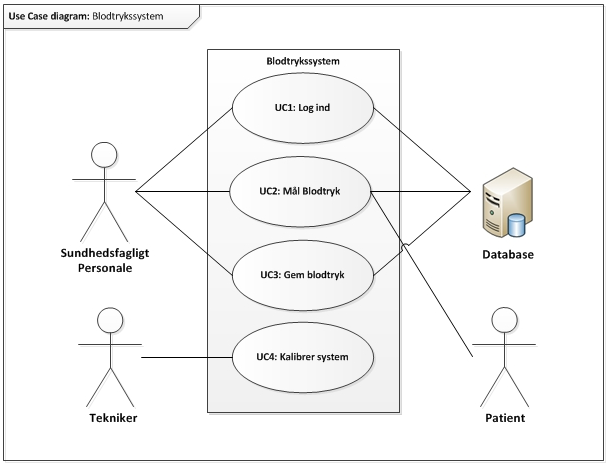
\includegraphics[scale=0.95]{uc.PNG}
\caption{Use case diagram}
\end{figure}

\subsection{Use case beskrivelser}


\subsubsection{Use case 1: Log ind}
For at kunne bruge systemet til blodtryksmåling, skal sundhedsfagligt personale logges ind. Dette gøres ved at indtaste korrekt ID med tilhørende kode, hvorefter der trykkes på "\textit{Log ind}"\- -knappen. Log ind-vinduet lukkes ned, og Diagnostik-vinduet vises. 


\subsubsection{Use case 2: Hent patientdata}
Før nulpunktsjusteringen kan foretages, skal patientens oplysninger angives. Dette gøres ved, at sundhedsfagligt personale indtaster patientens CPR-nummer og trykker på knappen "\textit{Hent patientoplysninger}"\- -knappen. Herefter angives patientens navn og CPR-nummer i Diagnostisk-vinduet. 

\subsubsection{Use case 3: Nulpunktsjustering}
Inden blodtryksmålingen kan foretages, skal systemet nulpunktsjusteres. Systemet foretager nulpunktsjustering efter at sundhedsfagligt personale har trykket på "\textit{Nulpunktsjustering}"\- -knappen. Herefter vises blodtrykket i Diagnostik-vinduet.

\subsubsection{Use case 4: Alarmer}
Systemet alarmerer sundhedsfagligt personale når blodtrykket bliver for højt eller lavt. Alarmeringen angives med lyd, hvorpå sundhedsfagligt personale har mulighed for at sætte systemets alarm på lydløs 

\subsubsection{Use case 5: Filtrer signal}
Sundhedsfagligt personale skal have mulighed for at slå det digitale filter til og fra. Dette gøres ved hjælp af "\textit{Til/fra}"\- -knappen.

\subsubsection{Use case 6: Gem data}
Systemet skal kunne gemme målingsdata. For at gemme data, trykker sundhedsfagligt personale på "\textit{Gem data}"\- -knappen, hvorefter måledata gemmes i databasen og systemet giver beskeden "\textit{Data gemt}"

\subsubsection{Use case 7: Kalibrer system}
Systemet kalibreres ved at tekniker påtrykker systemet tre kendte tryk. Herefter aflæser hen responserne på brugergrænsefladen og noterer afivgelserne fra de kendte tryk. Tekniker justerer så afvigelserne i systemets software, og systemet er kalibreret. 

\subsection{Fullydressed use case for use case X}
En direkte kopiering af tabellen fra Dokumentation, så ændringer fra ene dokument automatisk opdateres i andet.


\section{Systemarkitektur}
Også direkte kopieringer fra Dokumentation.

\subsection{Hardware}

\subsection{Software}


\section{Produktet}

Udarbejdelsen af produktet i hardware og software under iterationsprocessen med design, implementering og test.

\subsection{Hardware}

\subsection{Software}


\section{Accepttest}

For udvalgt use case.


\section{Opfyldelse af kravspecifikation}
Vurdering af accepttestens resultat.


\section{Videreudvikling}
Videreudvikling af selve produktet.


\backmatter
\chapter{Bilagsliste}\label{kapitel_Bilag}

Indsæt referencer til bilagene i Dokumentation.

\bibliography{bibliografi/PRJ3}    % Sætter bibliografien bagerst i dokumentet. Bruger bib-filen PRJ3.

\end{document}
